\section{Utilisateurs}
			Les utilisateurs peuvent commenter un produit une seule fois, mais peuvent répondre à un commentaire autant de fois que nécessaire.\\
			Ils peuvent effectuer des recherches sur le nom et les attributs (comme le prix) d'un produit pour pouvoir plus tard, l'acheter ou le louer.\\
			
		\section{Administrateur}
			L'administrateur est un utilisateur ayant le privilège d'acceder au panneau d'administrateur qui permet, à l'aide de php de manipuler la base de donnée.
		
		\section{Catégories}
			Les catégories possèdent catégories et produits, nous pouvons très bien avoir une sous-sous-sous-sous-sous-sous-sous-sous-catégorie contenant aucun produit, c'est possible, c'est à Brico-Bob de bien gérer cela.\\
			Le mieux étant de creer des catégories de catégories et des catégories de produits seulement, selon moi.
		\section{Flexibilité}
	
			\subsection{Changement du design du site}
	Si le client veut changer le design du site, il suffira de changer les fichiers .css ainsi que les images dans le dossier img. Par exemple pour changer les couleurs, la commande "remplacer tout" de notepad++ permettrait de changer les codes hexa assez rapidement.

\subsection{Type de matériel}
	Si le client veut que son site soit conçu pour une taille d'écran bien précise, il faudrait alors changer la taille de la page dans les fichiers ,css ainsi que d'agrandir certaines boites grâce a la propriété CSS width.

\subsection{Changement du contenu}
	Notre site est adapté au cas ou on voudrait changer son contenu. Si le client ne souhaite plus vendre de produits de bricolage, mais de l'électroménager.
Il suffirait de changer les noms des produits, catégories et de changer quelques images pour coller avec le nouveau thème du site.	

	\section{Portabilité}

\subsection{Différents navigateurs}

	Notre application est fonctionnelle sur les versions récentes de Google chrome, internet explorer et Firefox. Le site fonctionne également sur des versions un peu plus anciennes, par exemple sur IE6. ( Nous n'avons pas utilisé de HTML5 ). La différence est que les navigateurs un peu anciens ne reconnaissent pas certaines propriétés CSS3 utilisées par exemple box-shadow ou les effets de dégradé. Cependant, nous avons fait en sorte que l'affichage reste "décent", même si le site sera quelque peu moins beau.

\subsection{Javascript}

	Si le visiteur désactive le Javascript, le site ne sera pas moins fonctionnel, seulement, certains menus seront légèrement moins intuitifs et beaux. Il devra par exemple re-remplir tout le formulaire d'inscription si il fait une erreur mais cela ne changera rien au fait que l'inscription se déroulera normalement.
	
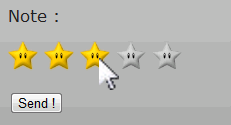
\includegraphics[scale=1]{exemplejs.png}